\chapter{Technology Evaluation}\label{techeval}
The technologies being used in this project are outlined below. \textcolor{red}{EXPAND}
\section{MongoDB}\label{mongo}
One of the most popular NoSQL technologies is MongoDB. MongoDB is an open source cross-platform DODB. The premise for using MongoDB is simplicity, speed and scalability (MongoDB White Paper, 2015). Its ever growing popularity, specifically amongst programmers, stems from the unrestrictive and flexible DODB data model which gives you the ability to query on all fields and boasts instinctive mapping of objects in modern programming languages. (MongoDB White Paper, 2015) The database design of MongoDB is based on the JSON file format named BSON. \begin{center}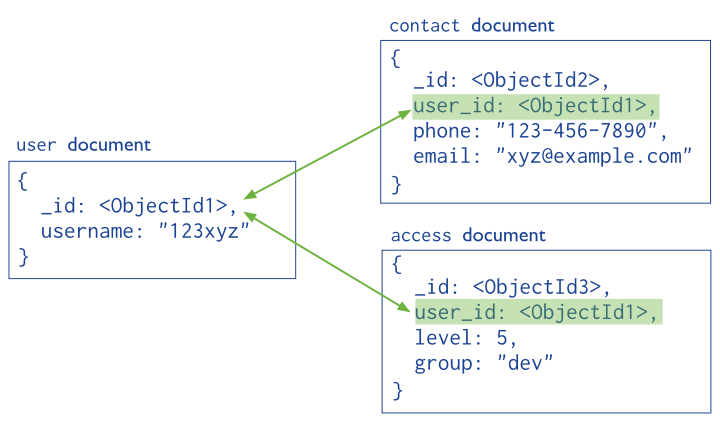
\includegraphics[width=1\linewidth]{images/mongodbmodel}\end{center}

*NOTES* A record in MongoDB is stored in collections. A collection is a grouping of MongoDB documents.
Within this free flowing environment documents can become as sophisticated and complex as required; information about a document record can be sub categorised by the integration of nested data. *NOTES*

\section{Neo4j}\label{neo}
Neo4j is an open-source NoSQL GODB which imposes the Property Graph Model throughout its implementation. The team behind the development of Neo4j describe it as an "An intuitive approach to data problems"(Neo4j web ref). One of the reasons in which Neo4j is favoured predominantly amongst database administrators and developers is its efficiency and high scalability. This is in part due to its compact storage and memory caching for the graphs. "Neo4j scales up and out, supporting tens of billions of nodes and relationships, and hundreds of thousands of ACID transactions per second."(Neo4j web ref) -\textcolor{red}{ FINISH WRITNG UP NOTES}

\section{Apache Cassandra}\label{cassandra}
Apache Cassandra, a top level Apache project born at Facebook and built on Amazon's Dynamo and Google's BigTable, is a distributed database for managing large amounts of structured data across many commodity servers, while providing highly available service and no single point of failure.  Cassandra offers capabilities that relational databases and other NoSQL databases simply cannot match such as: continuous availability, linear scale performance, operational simplicity and easy data distribution across multiple data centres and cloud availability zones.

\begin{center}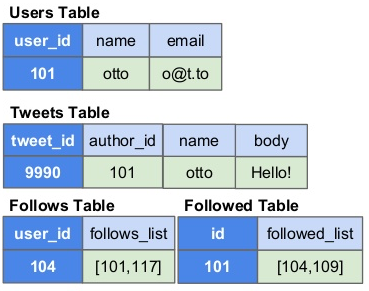
\includegraphics[width=0.75\linewidth]{images/cassandramodel}\end{center}

Cassandra's architecture is responsible for its ability to scale, perform, and offer continuous uptime. Rather than using a legacy master-slave or a manual and difficult-to-maintain shared architecture, Cassandra has a masterless "ring" design that is elegant, easy to setup, and easy to maintain.

\section{MySQL}\label{mysql}
MySQL is a freely available open source Relational Database Management System (RDBMS) that uses Structured Query Language (SQL).